\documentclass[10pt,a4paper]{article}
\usepackage[left=2.5cm,right=2.5cm,top=2.5cm,bottom=2.5cm,]{geometry}
\usepackage{amsmath,amssymb,amsthm}
\newtheorem{theorem}{Theorem}[section]
\newtheorem{lemma}[theorem]{Lemma}
\newtheorem{proposition}[theorem]{Proposition}
\usepackage{setspace}
\usepackage{graphicx}
\usepackage{lipsum}
\setlength{\parindent}{0pt}
\onehalfspacing
\usepackage{listings}
\usepackage{xcolor}
\lstset{
    basicstyle=\ttfamily\small,
    keywordstyle=\color{blue},
    commentstyle=\color{green!50!black},
    numbers=left,
    numberstyle=\tiny,
    frame=single,
    breaklines=true
}
\begin{document}
\section{BSDF}
BSDF carefully defines the reflective properties of object surfaces.
Before introducing BSDF, let's clarify two concepts.\\
The $irradiance$ describles the radiant flux reaching a unit area.
Simply, it describles actual light intensity received by the surface,(so it need $\cos$,ha?).\\
The $radiance$ describles radiant flux per unit projected area per unit solid angle.\\
The $differential irradiance$ describles the contribution of incident irradiance $L_i(\omega_i)$ from a specific direction $w_i$ to a point on the surface.
\[dE(\omega_i)=dL_i(\omega_i)\cos\theta d\omega_i\]
The $differential radiance$ describles the describles the emissivity of the incident direction $\omega_i$
in the reflective direction $\omega_o$.
\[L_o(\omega_o)=\int_{\Omega}dL_o(\omega_o)\]
Differential emissivity is proportional to differential irradiance, hence the definition of BSDF.
\[f_r(\omega_i,\omega_o)=\frac{dL_o(\omega_o)}{dL_i(\omega_i)\cos\theta d\omega_i}\cdot\frac{1}{\mathtt{sr}}\]
Naturally, we then wrote out the rendering equation.
\[L_o(\omega_o)\int_{\Omega}f_r(\omega_i,\omega_o)L_i(\omega_i)\cos\theta_i d\omega_i\cdot\frac{1}{\mathtt{sr}}\]
\subsection{Sampling based on Monte Carlo integral}
Monte Carlo integral is an efficent sample method. It's unbiased and the variance decreased to $\frac{1}{N^2}$. In rendering,it can be written by following style:
\[L_o(\omega_o)=L_e(\omega_o)+\frac{1}{N}\sum\limits_{i=1}^N\frac{f_r(\omega_i,\omega_oo)L_i(\omega_i)\cos\theta}{p(\omega_i)}\]
\begin{proposition}
    Monte Carlo integral is unbiased and the variance decreased  to $\frac{1}{N^2}$
\end{proposition}
\begin{proof}
    Let $g(\omega_i)=\frac{f_r(\omega_i,\omega_o)L_i(\omega_i)\cos\theta}{p(\omega_i)}$
    \[\mathbb{E}[g(\omega_i)]=\int_{\Omega}g(\omega_i)\cdot p(\omega_i)d\omega_i=\int_{\Omega}g(\omega_i)d\omega_i\]
    \[\mathbb{Var}[g(\omega_i)]=\mathbb{E}[g^2(\omega_i)]-\mathbb{E}[g^2(\omega_i)]\]
    \[\sigma=\int_{\Omega}\frac{g^2(\omega_i)}{p(\omega_i)}-\int_{\Omega}g^2(\omega_i)\]
    Because of the samples are independent and identically distributed.
    let: \[\mathbb{V}[ar]=\frac{\sigma}{N^2}\]
\end{proof}
Therefore, choosing a reasonable PDF is crucial. What is the best $p(\omega_i)$?\\
Let the optimal proposal distribution is $q(\omega_i)$.
\[I=\int g(\omega_i)p(\omega_i)d\omega_i\]
\[\mathbb{Var}[I]=\frac{1}{n}(\int\frac{g^2(\omega_i)p^2(\omega_i)}{q(\omega_i)}-I^2)d\omega_i\]
obviously we should minimize $\int\frac{g^2(\omega_i)p^2(\omega_i)}{q(\omega_i)}$\\
Constructing Lanrange multipliers.\[\mathcal{L}(\omega_i,\lambda)=\int(\frac{g^2(\omega_i)p^2(\omega_i)}{q(\omega_i)}+\lambda q(\omega_i))d\omega_i\]
Use the calculus of variations:
\[\frac{\partial(\frac{g^2p^2}{q}+\lambda q)}{\partial q}=-\frac{g^2p^2}{q}+\lambda=0\]
\[q(\omega_i)=\frac{|g(\omega_i)|p(\omega_i)}{\int|g(\omega_i)|p(\omega_i)d\omega_i}\]
unfortunately, this is incalaulate. The equation we want appear the answer. so we use sample.
\subsubsection{Cosnie-Weighted Hemisphere sampling}
In an ideal diffuse reflection model, $f_r=\frac{\rho}{\pi}$, this gives us a natural idea that let PDF be proportional to $\cos\theta$.
\[\int_{\Omega}p(\omega)d\omega=\int_{0}^{2\pi}\int_{0}^{\frac{\pi}{2}}(c\cdot\cos\theta)\sin\theta d\theta d\phi=1\]
\[p(\omega)=\frac{cos\theta}{\pi}\]
\[L_o(\omega_o)=\frac{\rho}{N}\sum\limits_{i=1}^{N}L_i(\omega_i)\]
It's unbiased. It quite obvious that it uses the idea of importance sampling--sample more from areas that makes a significant contributions.\\
A native way to implement this is use CDF's inverse function. 
\[\int_{0}^{2\pi}\int_{0}^{\frac{\pi}{2}}p(\theta,\phi)d\theta d\phi=\int_{0}^{2\pi}\int_{0}^{2\pi}p(\omega)d\theta d\phi=1\]
\[p(\theta)=\int_{0}^{2\pi}p(\phi)d\theta d\phi\]
\[F(\theta)=\int_{0}^{\theta}p(\theta)=\sin^2\theta\]
Give to random number $\xi_1,\xi_2\in[0,1]$
\[F(x)=\xi_1\to\sin\theta=\sqrt{\xi_1},\cos\theta=\sqrt{1-\xi_1}\]
\[x=\cos\theta\phi\sin\phi=\cos(2\pi\xi_2)\sqrt{\xi_1}\]
\[y=\sin\phi\sin\theta=\sin(2\pi\xi_2)\sqrt{xi_1}\]
\[z=\sqrt{1-\xi_1}\]
\begin{lstlisting}[language=C++]
template<typename T>
vec3<T,V>sp(const vec3<T,V>&n,int dep){
    Independent<T>s=in.clone(dep);
    T u=s.get1d(),v=s.get1d();T phi=2.0*3.1415926535*u;
    T r=sqrt(v);assert(!isnan(r));T x=cos(phi)*r,z=sin(phi)*r,y=sqrt(max(0.0,1.0-v));vec3<T,V>u1;
    if(abs(n.x)>T(0.1))u1=nor(cs(vec3<T,V>(0,1.0,0),n));
    else u1=nor(cs(vec3<T,V>(1.0,0,0),n));
    vec3<T,V>v1=cs(n,u1);return x*u1+y*n+z*v1;
}
\end{lstlisting}
\lipsum[1]
\begin{figure}[htbp]
    \centering
    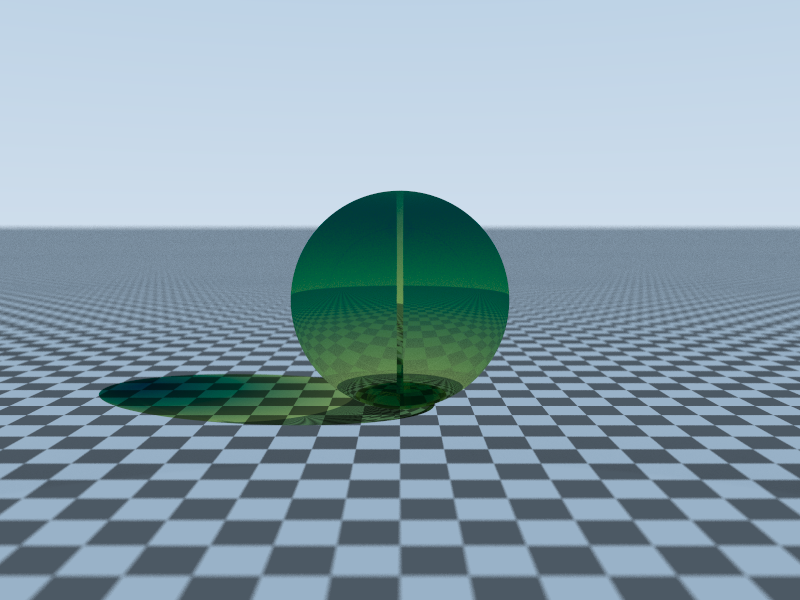
\includegraphics[width=\textwidth]{figures/brdf/a.png}
    \caption{100spp}
    \label{fig:ball}
\end{figure} 
Another way is uniform disk mapping, it's so easy to understand and implement. Not mentioned much(am I lazy? decided not to).
\subsubsection{Light source area sampling}
If the light is too small, the above method has very slow variance canvergence. Since sampling b=objects is slow, let's just sample the light soure directly.
For any pixel, we sample the light source and connect the pixel and the light source. But the problem is the  render equation is defined in the directional domain(soild angle). We need a concersion factor. What came to your mind? Jacobian. 
We need to project the surface area onto a plane perpendicular to light rays.
\[dA^\perp=dA\cos\theta_L\]
\[\frac{dA^\perp}{dA}=\cos\theta_L\]
distance scaling 
\[d\omega=\frac{dA^\perp}{r^2}\]
\[\frac{d\omega}{dA^\perp}=\frac{1}{r^2}\]
\[d\omega=(\frac{dA^\perp}{dA}\cdot\frac{d\omega}{dA^\perp})dA=\frac{\cos\theta_L}{r^2}dA\]
\[L_o(x,\omega_o)\approx\frac{A}{N}\sum\limits_{k=1}^{N}L_e(y_k\to x,-\omega_k)\cdot\frac{\cos\theta_L}{r^2}\cos\theta_k\cdot V(x,y_k)\]
where $V(x,y)$ is visable function and $p(\omega)=\frac{1}{A\cdot|J|}$
\begin{lstlisting}[language=C++]
template<typename T>
vec3<T,P>sun(5,5,5);
template<typename T>
vec3<T,P>p1(6,5,2);
template<typename T>
vec3<T,P>p2(3,7,4);
template<typename T>
Spectrum<T>sc(10,10,10);
template<typename T>
vec3<T,V>e1=p1<T>-sun<T>;
template<typename T>
vec3<T,V>e2=p2<T>-sun<T>;
template<typename T>
vec3<T,V>area(){
    sampler<T>s;
    T u=s.get1d(),v=s.get1d();vec3<T,V>rd=u*e1<T>+v*e2<T>;
    vec3<T,P>pt=sun<T>+vec3<T,P>(rd.x,rd.y,rd.z);
    vec3<T,V>dir=pt-p;vec3<T,V>n1=nor(cs(e1<T>,e2<T>));
    T s=len(cs(e1<T>,e2<T>));T dis=max(len(dir),eps);return nor(dir);
}
\end{lstlisting}
\begin{figure}[htbp]
    \centering
    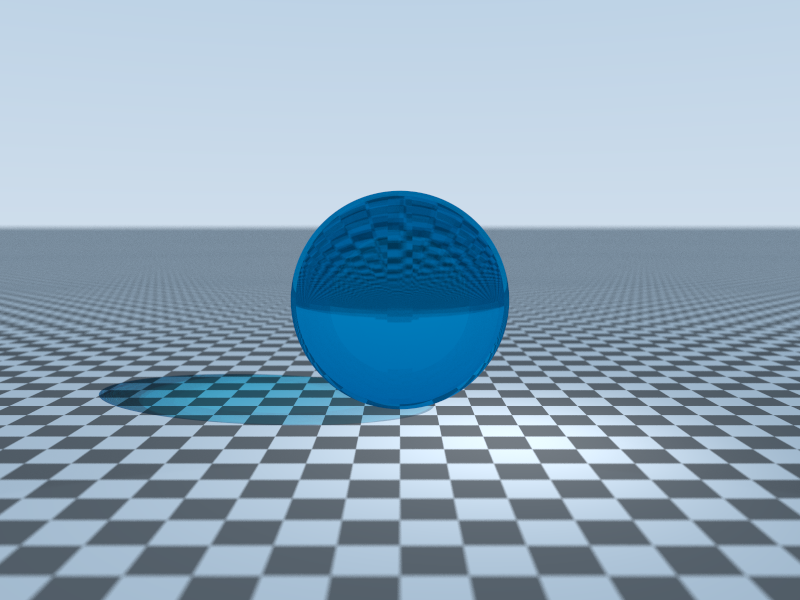
\includegraphics[width=\textwidth]{figures/brdf/b.png}
    \caption{light intensity:10 100spp}
    \label{fig:ball}
\end{figure}
\begin{figure}[htbp]
    \centering
    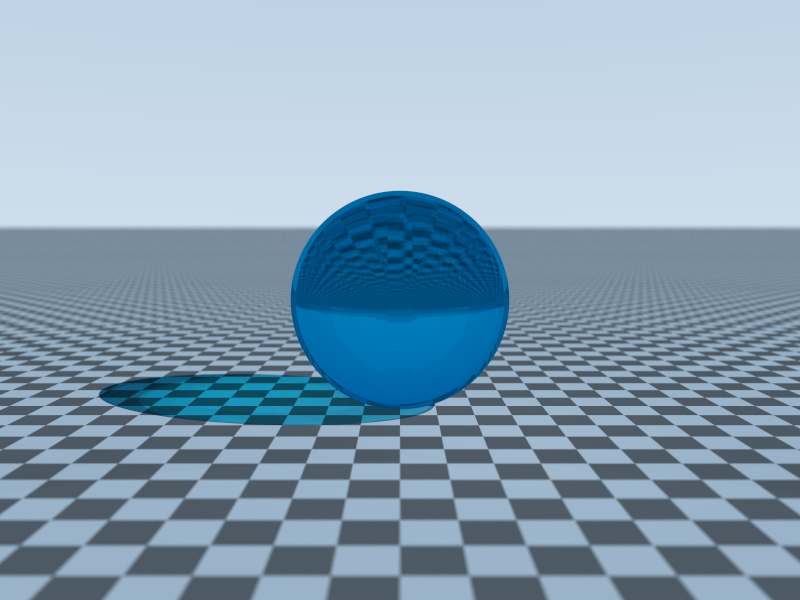
\includegraphics[width=\textwidth]{figures/brdf/c.png}
    \caption{light intensity:1 1024spp}
    \label{fig:ball}
\end{figure}
\end{document}
